\chapter{Linguaggi context-free}
In questo capitolo presentiamo grammatiche context-free, un metodo più potente per descrivere linguaggi. Queste grammatiche possono descrivere alcuni aspetti che hanno una struttura ricorsiva. Ciò le rende utili in una varietà di applicazioni.

Un'importante applicazione delle grammatiche context-free si presenta nella specifica e nella compilazione dei linguaggi di programmazione. Progettisti di compilatori e interpreti per linguaggi di programmazione spesso iniziano con l'ottenere una grammatica per il linguaggio. La maggior parte dei compilatori e degli interpreti contiene una componente chiamata parser che estrae il significato di un programma prima di generare il codice compilato o di eseguire il programma interpretato. Alcuni strumenti generano perfino automaticamente il parser dalla grammatica.

I linguaggi associati alle grammatiche context-free sono chiamati linguaggi context-free. La classe dei linguaggi context-free include tutti i linguaggi regolari e molti altri linguaggi.

\section{Grammatiche context-free}
Un esempio di grammatica context-free, che chiamiamo $G_{1}$ , è il seguente
\begin{gather*}
A\to 0A1\\
A\to B\\
B\to \#
\end{gather*}
Una grammatica consiste di un insieme di regole di sostituzione, anche chiamate produzioni. Ogni regola appare come una linea nella grammatica, costituita da un simbolo e una stringa separati da una freccia. Il simbolo è chiamato una variabile. La stringa consiste di variabili e altri simboli chiamati terminali. Le variabili sono spesso rappresentate da lettere maiuscole. I terminali sono analoghi ai simboli dell'alfabeto di input e sono spesso rappresentati da lettere minuscole, numeri o simboli speciali. Una delle variabili è chiamata la variabile iniziale. Essa generalmente si trova sul lato sinistro della regola più in alto. Per esempio, la grammatica $G_{1}$ ha tre regole. Le variabili di $G_{1}$ sono $A$ e $B$, e $A$ è la variabile iniziale. I suoi terminali sono 0, 1 e $\#$.

Una grammatica può essere usata per descrivere un linguaggio generando ogni stringa del linguaggio nel seguente modo.
\begin{enumerate}
    \item Scrivi la variabile iniziale. È la variabile sul lato sinistro della regola più in alto, a meno che non sia diversamente specificato.
    \item Trova una variabile che è stata scritta e una regola che inizia con quella variabile. Sostituisci la variabile scritta con il lato destro di quella regola.
    \item Ripeti il passo 2 fino a quando non vi sono più variabili.
\end{enumerate}
Per esempio, la grammatica $G_{1}$ genera la stringa $000\#111$. Una sequenza di sostituzioni per ottenere una stringa è chiamata una derivazione. Una derivazione della stringa $000\#111$ nella grammatica $G_{1}$ è:
\begin{equation*}
A\Rightarrow 0A1\Rightarrow 00A11\Rightarrow 000A111\Rightarrow 000B111\Rightarrow 000\#111
\end{equation*}
La stessa informazione può essere anche rappresentata mediante un disegno con un albero sintattico (parse tree - vedi Figura \ref{fig:parse-tree}).

\begin{figure}[ht]
    \centering
    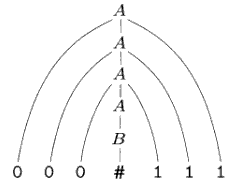
\includegraphics[width=0.3\linewidth]{images/parse-tree.png}
    \caption{Albero sintattico per \texttt{000\#111} nella grammatica $G_1$}
    \label{fig:parse-tree}
\end{figure}

Tutte le stringhe generate in questo modo costituiscono il linguaggio della grammatica. Denoteremo con $L(G_{1})$ il linguaggio della grammatica $G_{1}$. Alcune prove con la grammatica $G_{1}$ mostrano che $L(G_1)$ è $(0^n\#1^n| n \geq 0)$. Ogni linguaggio che può essere generato da una grammatica context-free è chiamato un linguaggio context-free (CFL). Nel presentare una grammatica context-free, è conveniente abbreviare le diverse regole con la stessa variabile a sinistra, come $A\to 0A1$ e $A\to B$ in una singola linea $A\to 0A1|B$, usando il simbolo "$|$" come un "oppure".

Formalizziamo la nostra nozione di grammatica context-free (CFG).

\begin{Definition}{Grammatica context-free}{}
Una grammatica context-free è una quadrupla $(V, \Sigma, R, S)$, dove

\begin{enumerate}
    \item $V$ è un insieme finito i cui elementi sono chiamati variabili,
    \item $\Sigma$ è un insieme finito, disgiunto da $V$, i cui elementi sono chiamati terminali,
    \item $R$ è un insieme finito di regole, dove ciascuna regola è una variabile e una stringa di variabili e terminali, ed
    \item $S\in V$ è la variabile iniziale.
\end{enumerate} 
\end{Definition}

Se $u$, $v$ e $w$ sono stringhe di variabili e terminali e $A\to w$ è una regola della grammatica, diciamo che $uAv$ produce $uwv$, e lo denotiamo con $uAv\Rightarrow uwv$. Diciamo che $u$ deriva $v$, e lo denotiamo con $u\Rightarrow v$ se $u = v$ o se esiste una sequenza $u_{1}, u_{2} ,...,u_k$ con $k\geq 0$ e
\begin{equation*}
u\Rightarrow u_1\Rightarrow u_2\Rightarrow...\Rightarrow u_k\Rightarrow v
\end{equation*}
Il linguaggio della grammatica è $\{ w\in\Sigma^*|S\Rightarrow^*w\}$.

Nella grammatica $G_{1}$: $V = \{A, B\}$ , $\Sigma=\{0, 1,\#\}$, $S = A$ ed $R$ è l'insieme delle tre regole.

\subsection{Progettare grammatiche context-free}
Come con la progettazione di automi finiti, la progettazione di grammatiche context-free richiede creatività. Le tecniche seguenti sono utili, singolarmente o combinate, quando affrontiamo il problema di costruire una CFG.

Innanzitutto, molti CFL sono l'unione di CFL più semplici. Se devi costruire una CFG per un CFL che puoi dividere in componenti più semplici, fallo e poi costruisci grammatiche separate per ciascuna componente. Queste singole grammatiche possono facilmente essere fuse in una grammatica per il linguaggio iniziale unendo le loro regole e poi aggiungendo la nuova regola $S\to S_{1}|S_{2}|...|S_k$ dove le variabili $S_{i}$ sono le variabili iniziali per le grammatiche individuali. Risolvere diversi problemi più semplici è spesso più facile che risolvere un problema complicato.

\begin{Example}{Grammatiche context-free - Unione}{}
Per esempio, per ottenere una grammatica per il linguaggio $\{0^n1^n|n\geq0\}\cup\{1^n0^n|n\geq0\}$ costruiamo prima la grammatica
\begin{equation*}
    S_{1}\to 0S_1 1|\epsilon    
\end{equation*}
per il linguaggio $\{0^n1^n|n\geq0\}$ e la grammatica
\begin{equation*}
    S_{2}\to 1S_2 0|\epsilon    
\end{equation*}
per il linguaggio $\{1^n0^n|n\geq0\}$ e poi aggiungiamo la regola $S\to S_1 |S_2$ ottenendo la grammatica
\begin{gather*}
    S\to S_1|S_2\\
    S_{1}\to 0S_1 1|\epsilon\\
    S_{2}\to 1S_2 0|\epsilon
\end{gather*}
\end{Example}

In secondo luogo, costruire una CFG per un linguaggio che sia regolare è facile se si può prima costruire un DFA per quel linguaggio. Si può trasformare un DFA in una CFG equivalente nel modo seguente. Si introduca una variabile $R_{i}$ per ogni stato $q_{i}$ del DFA. Si aggiunga la regola $R_{i}\to aR_{j}$ alla CFG se $\delta(q_{i}, a) = q_{j}$ è una transizione nel DFA. Si aggiunga la regola $R_{i}\to\epsilon$ se $q_{i}$ è uno stato accettante del DFA. Si assuma $R_{0}$ come variabile iniziale della grammatica, dove $q_{0}$ è lo stato iniziale della macchina. Si può verificare che la CFG risultante genera lo stesso linguaggio di quello riconosciuto dal DFA.

Inoltre, alcuni linguaggi context-free contengono stringhe con due sottostringhe che sono "collegate", nel senso che una macchina per un tale linguaggio avrebbe bisogno di ricordare una quantità non limitata di informazione su una delle sottostringhe per verificare che essa corrisponde correttamente all'altra sottostringa. Questa situazione si verifica nel languaggio $\{0^n1^n|n\geq0\}$ poiché una macchina avrebbe bisogno di ricordare il numero di uguali a 0 per verificare che esso è uguale al numero di simboli uguali a 1. Si può costruire una CFG per gestire questa situazione usando una regola della forma $R\to uRv$ che genera stringhe nelle quali la porzione contenente le $u$ corrisponde alla porzione contenente le $v$.

Infine, in linguaggi più complessi, le stringhe possono contenere alcune strutture che compaiono ricorsivamente come parte di altre strutture (o della stessa).

\subsection{Ambiguità}
Qualche volta una grammatica può generare la stessa stringa in più modi diversi. Una tale stringa avrà diversi alberi sintattici e quindi diversi significati.

Se una grammatica genera la stessa stringa in più modi diversi, diciamo che la stringa è derivata ambiguamente in quella grammatica. Se una grammatica genera alcune stringhe ambiguamente, diciamo che la grammatica è ambigua.

\begin{Example}{Grammatica ambigua}{}
Per esempio, consideriamo la grammatica:
\begin{equation*}
    E\to E + E | E\times E | (E) | a
\end{equation*}
Questa grammatica genera la stringa $a+a\times a$ ambiguamente. La figura seguente mostra i due diversi alberi sintattici.

\begin{minipage}{\textwidth}
    \centering
    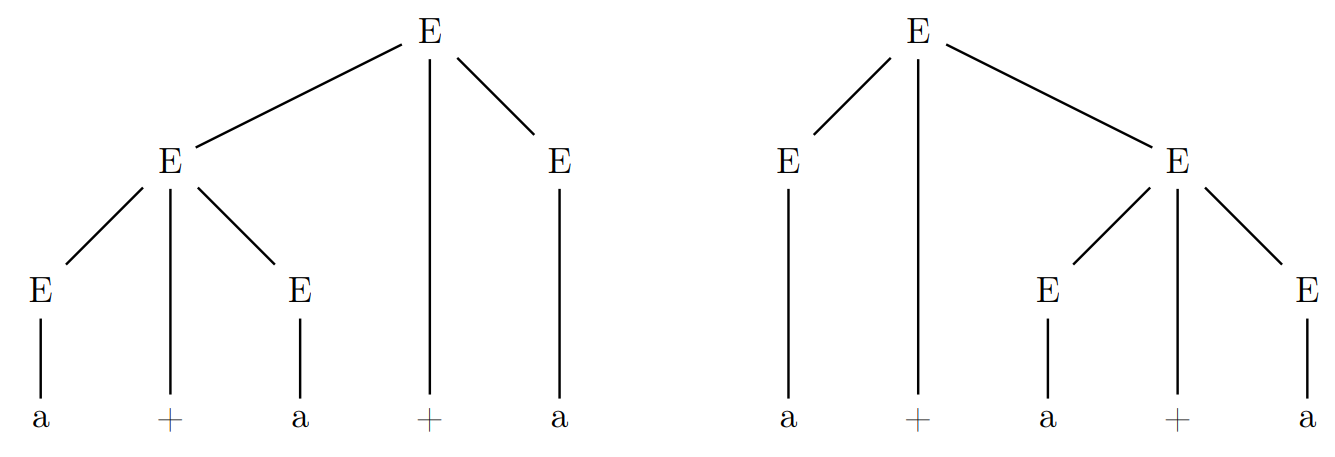
\includegraphics[width=0.7\textwidth]{images/es-alberi-sintattici.PNG}
    %\captionof{figure}{Diagramma di stato per un automa finito $M_2$}
\end{minipage}
\end{Example}

Questa grammatica non tiene conto delle usuali regole di precedenza e quindi può raggruppare $+$ prima di $\times$ o viceversa.

Ora formalizziamo la nozione di ambiguità. Quando diciamo che una grammatica genera ambiguamente una stringa, intendiamo che la stringa ha due diversi alberi sintattici, non due differenti derivazioni. Due derivazioni possono differire solo nell'ordine in cui esse sostituiscono le variabili ma non nella loro struttura complessiva. Per concentrarci sulla struttura, definiamo un tipo di derivazione che sostituisce le variabili con un ordine stabilito. Una derivazione di una stringa $w$ in una grammatica $G$ è una derivazione a sinistra (leftmost derivation) se a ogni passo la variabile sostituita è quella che si trova più a sinistra.

\begin{Definition}{Derivazione ambigua}{}
Una stringa $w$ è derivata ambiguamente in una grammatica context-free $G$ se essa ha due o più diverse derivazioni a sinistra. Una grammatica $G$ è ambigua se essa genera qualche stringa ambiguamente.
\end{Definition}

Qualche volta quando abbiamo una grammatica ambigua, possiamo trovare una grammatica non ambigua che genera lo stesso linguaggio. Tuttavia, alcuni linguaggi context-free possono essere generati solo da grammatiche ambigue. Tali linguaggi sono chiamati inerentemente ambigui.

\subsection{Forma normale di Chomsky}
Quando si lavora con le grammatiche context-free, è spesso conveniente averle in forma semplificata. Una delle forme più semplici e utili è chiamata la forma normale di Chomsky. La forma normale di Chomsky è utile nel dare algoritmi che lavorano con grammatiche context-free.

\begin{Definition}{Forma normale di Chomsky}{}
Una grammatica context-free è in forma normale di Chomsky se ogni regola è della forma
\begin{gather*}
    A\to BC\\
    A\to a
\end{gather*}
dove $a$ è un terminale e $A$, $B$ e $C$ sono variabili qualsiasi tranne che $B$ e $C$ non possono essere la variabile iniziale. Inoltre, permettiamo la regola $S\to \epsilon$, dove $S$ è la variabile iniziale.
\end{Definition}

\begin{Thm}{CFG in forma normale di Chomsky}{}\label{thm:cfg-chomsky}
\textit{Ogni linguaggio context-free è generato da una grammatica context-free in forma normale di Chomsky.}
\begin{osservation}
Possiamo trasformare ogni grammatica $G$ in forma normale di Chomsky. La trasformazione ha diversi passi nei quali le regole che violano le condizioni sono rimpiazzate con regole equivalenti che sono adeguate. Innanzitutto, aggiungiamo una nuova variabile iniziale. Poi, eliminiamo tutte le $\epsilon$-regole della forma $A\to\epsilon$. Eliminiamo anche tutte le regole unitarie della forma $A\to B$ In entrambi i casi, modifichiamo la grammatica in modo da essere sicuri che generi ancora lo stesso linguaggio. Infine, trasformiamo le restanti regole nella forma adeguata.
\end{osservation}
\begin{demonstration}
In primo luogo, aggiungiamo una nuova variabile iniziale $S_{0}$ e la regola $S_{0}\to S$ dove $S$ era la variabile iniziale di partenza. Questo cambiamento garantisce che la variabile iniziale non compare sul lato destro di una regola.

In secondo luogo, ci occupiamo di tutte le $\epsilon$-regole. Eliminiamo una $\epsilon$-regola $A\to\epsilon$ dove $A$ non è la variabile iniziale. Poi, per ogni occorrenza di $A$ sul lato destro di una regola, aggiungiamo una nuova regola con quell'occorrenza cancellata. In altre parole, se $R\to uAv$ è una regola in cui $u$ e $v$ sono stringhe di variabili e terminali, aggiungiamo la regola $R\to uv$. Facciamo questo per ogni occorrenza di $A$, in modo che la regola $R\to uAvAw$ faccia si che vengano aggiunte $R\to uvAw$, $R\to uAvw$ ed $R\to uvw$. Se abbiamo la regola $R\to A$ aggiungiamo $R\to\epsilon$ a meno che non avevamo precedentemente rimosso la regola $R\to\epsilon$. Ripetiamo questi passi fino a eliminare tutte le $\epsilon$-regole che non coinvolgono la variabile iniziale.

Inoltre, ci occupiamo delle regole unitarie. Eliminiamo una regola unitaria $A\to B$. Poi, per ogni regola $B\to u$ aggiungiamo la regola $A\to u$ a meno che questa non sia una regola unitaria precedentemente cancellata. Come prima, $u$ è una stringa di variabili e terminali. Ripetiamo questi passi fino a eliminare tutte le regole unitarie.

Infine, trasformiamo tutte le restanti regole nella forma appropriata. Rimpiazziamo ogni regola $A\to u_{1}u_{2}...u_k$, dove $k\geq 3$ e ciascun $u_{i}$ è una variabile o un simbolo terminale, con le regole $A\to u_{1}A_{1}$, $A_{1} \rightarrow u_{2}A_{2}$, $A_{2}\to u_{3}A_{3}$,... and $A_{k-2}\to u_{k-1}u_k$. Le $A_{i}$ sono nuove variabili. Rimpiazziamo ogni terminale $u_{i}$ nelle precedenti regole (o regola) con la nuova variabile $U_{i}$ e aggiungiamo la regola $U_{i}\to u_{i}$.
\end{demonstration}
\end{Thm}

\begin{Example}{Trasformazione CFG in forma normale di Chomsky}{}
\textit{Consideriamo la seguente CFG $C_6$ e trasformiamola in forma normale di Chomsky.}
    
La sequenza di grammatiche presentate illustra i passi nella conversione.
\begin{enumerate}
    \item La CFG iniziale $G_{6}$ è mostrata sulla sinistra. Il risultato dell'applicazione del primo passo, che crea una nuova variabile iniziale, è mostrato sulla destra.
    
    \begin{minipage}{0.49\textwidth}
    \begin{gather*}
        S\to ASA |aB\\
        A\to B|S\\
        B\to b|\epsilon
    \end{gather*}
    \end{minipage}
    \begin{minipage}{0.49\textwidth}
    \begin{gather*}
        S_0\to S\\
        S\to ASA|aB\\
        A\to B|S\\
        B\to b|\epsilon
    \end{gather*}    
    \end{minipage}
    \item Eliminiamo le $\epsilon$-regole $B\to \epsilon$ come mostrato sulla sinistra, e $A\to\epsilon$ come mostrato sulla destra.
    
    \begin{minipage}{0.49\textwidth}
    \begin{gather*}
        S_0\to S\\
        S\to ASA|ab|a\\
        A\to B|S|\epsilon\\
        B\to b|\cancel{\epsilon}
    \end{gather*}
    \end{minipage}
    \begin{minipage}{0.49\textwidth}
    \begin{gather*}
        S_0\to S\\
        S\to ASA|aB|a|SA|AS|S\\
        A\to B|S|\cancel{\epsilon}\\
        B\to b
    \end{gather*}    
    \end{minipage}
    \item[3a.] Eliminiamo le regole unitarie $S\to S$ come mostrato sulla sinistra, e $S_{0}\to S$ come mostrato sulla destra.

    \begin{minipage}{0.49\textwidth}
    \begin{gather*}
        S_0\to S\\
        S\to ASA|aB|a|SA|AS|\cancel{S}\\
        a\to B|S\\
        B\to b
    \end{gather*}
    \end{minipage}
    \begin{minipage}{0.49\textwidth}
    \begin{gather*}
        S_0\to \cancel{S}|ASA|aB|a|SA|AS\\
        S\to ASA|aB|a|SA|AS\\
        A\to B|S\\
        B\to b
    \end{gather*}    
    \end{minipage}
    \item[3b.] Eliminiamo le regole unitarie $A\to B$ e $A\to S$.

    \begin{minipage}{0.49\textwidth}
    \begin{gather*}
        S_0\to ASA|aB|a|SA|AS\\
        S\to ASA|aB|a|SA|AS\\
        A\to \cancel{B}|\cancel{S}|b\\
        B\to b
    \end{gather*}
    \end{minipage}
    \begin{minipage}{0.49\textwidth}
    \begin{gather*}
        S_0\to ASA|aB|a|SA|AS\\
        S\to ASA|aB|a|SA|AS\\
        A\to S|b|ASA|aB|a|SA|AS\\
        B\to b
    \end{gather*}    
    \end{minipage}
    \item[4.] Trasformiamo le rimanenti regole nella forma corretta, aggiungendo variabili e regole supplementari. La grammatica finale in forma normale di Chomsky è equivalente a $G_{6}$ (In realtà la procedura fornita nel Teorema \ref{thm:cfg-chomsky} crea diverse variabili $U_i$ e diverse regole $U_i\to a$. Abbiamo semplificato la grammatica risultante usando una sola variabile $U$ e una sola regola $U\to a$).
    \begin{gather*}
        S_0\to AA_1|UB|a|SA|AS\\
        S\to AA_1|UB|a|SA|AS\\
        A\to b|AA_1|UB|a|SA|AS\\
        A_1\to SA\\
        U\to a\\
        B\to b
    \end{gather*}
\end{enumerate}    
\end{Example}

\section{Automi a pila}
In questa sezione introduciamo un nuovo tipo di modello computazionale chiamato automa a pila (pushdown automata). Questi automi sono come gli automi finiti non deterministici ma hanno una componente in più chiamata pila (stack). La pila fornisce memoria aggiuntiva oltre alla quantità finita di essa disponibile nel controllo. La pila consente a tali automi di riconoscere alcuni linguaggi non regolari.

Gli automi a pila sono computazionalmente equivalenti alle grammatiche context-free. Questa equivalenza è utile poiché essa ci dà due alternative per provare che un linguaggio è context free. Possiamo dare una grammatica context-free che lo genera oppure un automa a pila che lo riconosce. Alcuni linguaggi sono più facilmente descritti in termini di generatori, mentre altri sono più facilmente descritti da riconoscitori.

Un automa a pila (PDA) può scrivere simboli nella pila e rileggerli in seguito. Scrivere un simbolo "spinge giù" tutti gli altri simboli nella pila. In un qualunque momento il simbolo sulla cima (top) della pila può essere letto e rimosso. I rimanenti simboli allora ritornano più in alto. L'operazione di scrivere un simbolo sulla pila è spesso chiamata push, quella di eliminare un simbolo dalla pila è spesso chiamata pop. Nota che ogni accesso alla pila, sia per leggere che per scrivere, può essere fatto solo sulla sommità. In altre parole, una pila è un dispositivo di memoria "last in, first out" (ultimo entrato, primo uscito). Se alcuni dati sono scritti nella pila e dati aggiuntivi sono scritti in seguito, i dati precedenti diventano inaccessibili fino a quando quelli successivi vengono rimossi.

Una pila è molto importante perché può mantenere una quantità non limitata di informazioni. Quindi, la natura non limitata di una pila permette al PDA di memorizzare numeri di dimensioni non limitate. La seguente descrizione informale mostra come opera l'automa per questo linguaggio.

\subsection{Definizione formale di automa a pila}
La definizione di automa a pila è simile a quella di un automa finito, tranne che per la pila. La pila è un dispositivo che contiene simboli presi da un qualche alfabeto. La macchina può usare differenti alfabeti per il suo input e la sua pila, quindi ora specifichiamo sia un alfabeto di simboli di input $\Sigma$ sia un alfabeto di pila $\Gamma$.

Nel cuore di ogni definizione di automa c'è la funzione di transizione, che descrive il suo comportamento. Ricordiamo che $\Sigma_\epsilon = \Sigma\cup\{\epsilon\}$ e $\Gamma_\epsilon = \Gamma\cup\{\epsilon\}$. Il dominio della funzione di transizione è $Q \times \Sigma_\epsilon \times \Gamma_\epsilon$. Quindi lo stato corrente, il prossimo simbolo di input letto, e il simbolo sulla cima della pila determinano la mossa seguente di un automa a pila. L'uno o l'altro simbolo può essere $\epsilon$, il che determina che la macchina si muova senza leggere un simbolo di input o senza leggere un simbolo dalla pila. 

Per quanto riguarda il codominio della funzione di transizione, dobbiamo considerare cosa può fare l'automa quando è in una specifica situazione. Esso può trovarsi in un nuovo stato ed eventualmente scrivere un simbolo sulla cima della pila. La funzione $\delta$ può indicare quest'azione restituendo un elemento di $Q$ insieme a un elemento di $\Gamma_\epsilon$, cioè un elemento di $Q\times\Gamma_\epsilon$. Poiché permettiamo il non determinismo in questo modello, una situazione può avere diverse mosse successive lecite. La funzione di transizione ingloba il non determinismo nel modo usuale, restituendo un insieme di elementi di $Q\times\Gamma_\epsilon$, cioè un elemento di $\mathcal{P}(Q\times \Gamma_\epsilon$). Mettendo tutto questo insieme, la nostra funzione di transizione $\delta$ assume la forma $\delta: Q\times\Sigma_\epsilon\times \Gamma_\epsilon\longrightarrow \mathcal{P}(Q\times \Gamma_\epsilon)$.

\begin{Definition}{Automa a pila}{}
Un automa a pila è una sestupla $(Q, \Sigma, \Gamma, \delta, q_{0}, F)$ dove $Q$, $\Sigma$, $\Gamma$ ed $F$ sono tutti insiemi finiti, e
\begin{enumerate}
    \item $Q$ è l'insieme degli stati,
    \item $\Sigma$ è l'alfabeto dell'input,
    \item $\Gamma$ è l'alfabeto della pila,
    \item $\delta: Q\times\Sigma_\epsilon\times \Gamma_\epsilon\longrightarrow \mathcal{P}(Q\times \Gamma_\epsilon)$ è la funzione di transizione.
    \item $q_{0}\in Q$ è lo stato iniziale, ed
    \item $F\subseteq Q$ l'insieme degli stati accettanti.
\end{enumerate}
\end{Definition}

Dato $(q, c)\in\delta(p, a, b)$ dove $\delta$ è la funzione di transizione di un PDA, si ha che:
\begin{itemize}
    \item Se $b, c = \epsilon$ (dunque $a; \epsilon \to\epsilon$) allora l’automa leggerà $a$ dalla stringa e passerà direttamente dallo stato $p$ allo stato $q$, senza modificare lo stack;
    \item Se $b = \epsilon$ e $c\neq\epsilon$ (dunque $a; \epsilon \to c$) allora l’automa leggerà $a$ dalla stringa, passerà direttamente dallo stato $p$ allo stato $q$ e in cima allo stack viene aggiunto il simbolo $c$ (push);
    \item Se $b\neq \epsilon$ e $c = \epsilon$ (dunque $a; b \to\epsilon$) allora l’automa leggerà $a$ e se in cima allo stack vi è $b$, l’automa passerà dallo stato $p$ allo stato $q$ e rimuoverà $b$ dalla cima dello stack (pop).
\end{itemize}
Un automa a pila $M = (Q, \Sigma, \Gamma, \delta, q_{0}, F)$ computa come segue. Accetta un input $w$ se $w$ può essere $w= w_{1}w_{2}...w_m$, dove ciascun $w_{i} \in \Sigma_{\epsilon}$ ed esistono sequenze di stati $r_{0}, r_{1} ,...,r_{m}\in Q$ di stringhe $s_{0}, s_{1} ,...,s_m\in \Gamma^*$ che soddisfano le tre condizioni seguenti. Le stringhe $s_{i}$ rappresentano la sequenza del contenuto della pila che $M$ ha su un ramo accettante della computazione.
\begin{enumerate}
    \item $r_{0} = q_{0}$ and $s_{0} = \epsilon$. Questa condizione significa che $M$ inizia correttamente, nello stato iniziale e con una pila vuota.
    \item Per $i = 0 ,...,m-1$ abbiamo $(r_{i+1}, b)\in\delta(r_i, w_{i+1}, a)$, dove $s_{i} = at$ ed $s_{i+1}=bt$ qualche $a,b\in\Gamma_\epsilon$ e $t\in\Gamma^*$. Questa condizione che muove correttamente in base allo stato, al simbolo di pila, e al prossimo simbolo in input.
    \item $r_{m} \in F$. Questa condizione afferma che alla fine dell'input $M$ si trova in uno stato accettante.
\end{enumerate}

\begin{Example}{Automa a pila}{}
\textit{Descrivere un PDA che riconosce il linguaggio $L=\{0^n1^n|n\geq0\}$.}

Un PDA è in grado di riconoscere questo linguaggio poiché può usare la sua pila per memorizzare il numero di simboli uguali a 0 che ha visto.

Legge i simboli in input. Scrive ciascun 0 letto sulla pila. Non appena vede simboli uguali a 1, cancella uno 0 dalla pila per ogni 1 letto. Se la lettura dell'input termina esattamente quando la pila diventa priva di simboli uguali a 0, accetta l'input. Se la pila si svuota ma restano simboli uguali a 1 o se i simboli uguali a 1 sono finiti ma la pila contiene ancora simboli uguali a 0 o se qualche 0 appare nell'input dopo i simboli uguali a 1, rifiuta l'input.

\begin{minipage}{\textwidth}
    \centering
    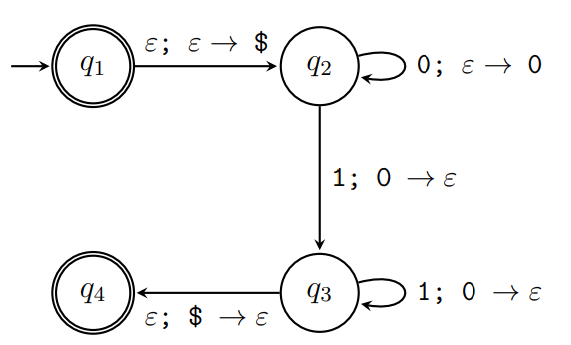
\includegraphics[width=0.4\textwidth]{images/es-automa-pila1.PNG}
    %\captionof{figure}{Diagramma di stato per un automa finito $M_2$}
\end{minipage}
\end{Example}

\begin{Example}{Automa a pila}{}
\textit{Descrivere un PDA che riconosce il linguaggio $L=\{ww^\mathcal{R}\}|w\in\{0, 1\}^*\}$.}

Ricordiamo che $w ^ \mathcal{R}$ significa $w$ scritta al contrario.

Inizia inserendo nella pila i simboli letti. In qualunque momento ipotizza non deterministicamente di aver raggiunto la prima metà della stringa e quindi cambia azione, eliminando dalla pila un simbolo per ciascun simbolo letto, se essi coincidono. Se essi coincidono sempre e la pila si svuota nello stesso momento in cui l'input è terminato, accetta; altrimenti rifiuta.

\begin{minipage}{\textwidth}
    \centering
    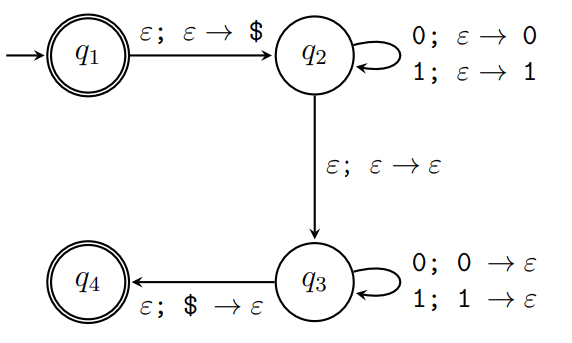
\includegraphics[width=0.4\textwidth]{images/es-automa-pila2.PNG}
    %\captionof{figure}{Diagramma di stato per un automa finito $M_2$}
\end{minipage}
\end{Example}

\subsection{Equivalenza con le grammatiche context-free}
Ora mostriamo che grammatiche context-free e automi a pila sono computazionalmente equivalenti. Entrambi sono in grado di descrivere la classe dei linguaggi context-free. Mostreremo come trasformare ogni grammatica context-free in un automa a pila che riconosce lo stesso linguaggio e viceversa. Ricordiamo che abbiamo definito un linguaggio context-free come un linguaggio che può essere descritto con una grammatica context-free. Quindi, il nostro obiettivo è il teorema seguente.

\begin{Thm}{Linguaggio context-free e automa a pila}{}\label{thm:cfa-implica-pda}
\textit{Un linguaggio è context-free se e solo se esiste un automa a pila che lo riconosce.}    
\end{Thm}

Come al solito, per i teoremi "se e solo se", abbiamo due enunciati da provare, nelle due direzioni. Innanzitutto trattiamo la direzione più facile, la diretta.

\begin{Lemma}{Linguaggio context-free implica automa a pila}{}\label{lemma:cfa-implica-pda}
\textit{Se un linguaggio è context-free, allora esiste un automa a pila che lo riconosce.}

\begin{osservation}
Sia $A$ un CFL. Dalla definizione sappiamo che esiste una CFG, $G$, che genera $A$. Mostriamo come trasformare $G$ in un PDA equivalente, che chiamiamo $P$.

Il PDA $P$ che ora descriviamo, opererà accettando il suo input $w$, se $G$ genera tale input, determinando se esiste una derivazione per $w$. Ricordiamo che una derivazione è semplicemente la sequenza di sostituzioni fatte nel processo di generazione di una stringa mediante una grammatica. Ogni passo di una derivazione produce una stringa intermedia di variabili e terminali. Noi progettiamo $P$ in modo che possa stabilire se una serie di sostituzioni che usano le regole di $G$ possa condurre dalla variabile iniziale a $w$.

Il non determinismo di un PDA gli consente di ipotizzare la sequenza di sostituzioni giuste. In ogni passo della derivazione, una delle regole per una particolare variabile è scelta non deterministicamente e usata per sostituire quella variabile.

Il PDA $P$ inizia scrivendo la variabile iniziale sulla sua pila. Esso passa attraverso una serie di stringhe intermedie, facendo una sostituzione dietro l'altra. Infine può giungere a una stringa che contiene solo simboli terminali, il che significa che ha usato la grammatica per derivare una stringa. Allora $P$ accetta se questa stringa è identica alla stringa che ha ricevuto in input.% Implementare questa strategia su un PDA richiede un'idea supplementare.

Il PDA può accedere solo al simbolo sulla cima della pila e questo potrebbe essere un simbolo terminale e non una variabile. Il modo per aggirare questo problema è mantenere solo parte della stringa intermedia sulla pila: i simboli che iniziano con la prima variabile nella stringa intermedia. Tutti i simboli terminali che compaiono prima della prima variabile sono subito abbinati con i simboli nella stringa di input.

\begin{enumerate}
    \item Inserisce il simbolo marcatore \$ e la variabile iniziale sulla pila.
    \item Ripete i seguenti passi.
    \begin{enumerate}
        \item Se sulla cima della pila c'è il simbolo di una variabile $A$, sceglie non deterministicamente una delle regole per $A$ e sostituisce $A$ con la stringa sul lato destro della regola.
        \item Se sulla cima della pila c'è un simbolo terminale $a$, legge il simbolo seguente dall'input e lo confronta con $a$. Se essi sono uguali, ripete. Se essi non sono uguali, rifiuta su questo ramo del non determinismo. 
        \item Se sulla cima della pila c'è il simbolo \$, entra nello stato accettante. In questo modo accetta l'input se esso è stato completamente letto.
    \end{enumerate}
\end{enumerate}

\begin{demonstration}
Ora diamo i dettagli formali della costruzione dell'automa a pila $P = (Q,\Sigma, \Gamma, \delta, q_{start}, F)$. Per rendere più chiara la costruzione, usiamo una notazione abbreviata per la funzione di transizione.

Siano $q$ ed $r$ stati del PDA e siano $a \in \Sigma_\epsilon$, ed $s\in\Gamma_\epsilon$. Supponiamo di volere che il PDA vada da $q$ a $r$ quando legge $a$ ed elimina $s$. Inoltre, vogliamo che esso inserisca l'intera stringa $u=u_1...u_l$ sulla pila simultaneamente. Possiamo eseguire questa azione introducendo nuovi stati $q_1, ..., q_{l-1}$ definendo la funzione di transizione come segue:
\begin{gather*}
\delta(q, a, s)\textit{ contiene }(q_1, u_l),\\
\delta(q_1, \epsilon, \epsilon)=\{(q_2, u_{l-1})\},\\
\delta(q_2, \epsilon, \epsilon)=\{(q_3, u_{l-2})\},\\
...\\
\delta(q_{l-1}, \epsilon, \epsilon)=\{(r, u_1)\}
\end{gather*}

Useremo la notazione $(r, u)$ e $\delta(q, a, s)$ per denotare che quando $q$ è lo stato in cui si trova l'automa, $a$ è il prossimo simbolo di input ed $s$ è il simbolo sulla cima della pila, il PDA può leggere $a$ ed eliminare $s$, poi inserire la stringa $u$ nella pila e passare nello stato $r$. La figura seguente ne mostra la realizzazione.

\begin{minipage}{\textwidth}
    \centering
    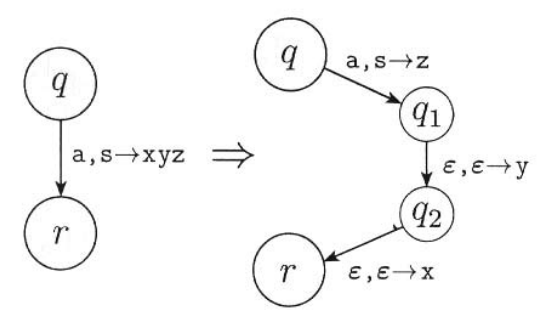
\includegraphics[width=0.4\textwidth]{images/CFG-implica-PDA.png}
    %\captionof{figure}{Diagramma di stato per un automa finito $M_2$}
\end{minipage}

Gli stati di $P$ sono $Q =\{q_{start}, q_{loop}, q_{accept}\}\cup E$, dove $E$ è l'insieme degli stati necessari per realizzare l'abbreviazione appena descritta. Lo stato iniziale è $q_{start}$. L'unico stato accettante è q$_{accept}$.

La funzione di transizione è definita come segue. Cominciamo inizializzando la pila inserendo i simboli \$ and $S$, realizzando così il passo 1 nella descrizione informale: $\delta(q_{start}, \epsilon, \epsilon)=\{(q_{loop}, S\$)\}$ Poi aggiungiamo le transizioni per il ciclo principale del passo 2.

In primo luogo, trattiamo il caso (a) in cui la cima della pila contiene una variabile. Poniamo $\delta(q_{loop}, \epsilon,A)=\{(q_{loop},w)| \textit{ dove } A\to w \textit{ è una regola in } R\}$.

In secondo luogo, trattiamo il caso (b) in cui la cima della pila contiene un terminale. Poniamo $\delta(q_{loop},a,a)=\{(q_{loop}, \epsilon)\}$.

Infine, trattiamo il caso scelto per indicare la pila vuota \$ è sulla cima della pila. Poniamo $\delta(q_{loop}, \epsilon,\$)=\{(q_{accept}, \epsilon)\}$.

\begin{minipage}{\textwidth}
    \centering
    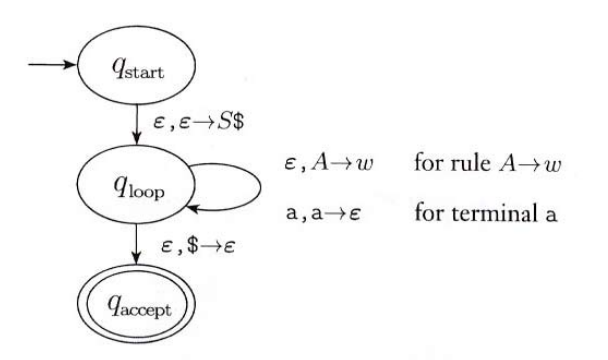
\includegraphics[width=0.5\textwidth]{images/CFG-implica-PDA2.png}
    %\captionof{figure}{Diagramma di stato per un automa finito $M_2$}
\end{minipage}
\end{demonstration}
\end{osservation}
\end{Lemma}

\begin{Example}{Linguaggio context-free implica automa a pila}{}
Usiamo la procedura sviluppata nel Lemma \ref{lemma:cfa-implica-pda} per costruire una PDA dalla seguente CFG $G$:
\begin{gather*}
    S\to aTb|b\\
    T\to Ta|\epsilon
\end{gather*}

\begin{minipage}{\textwidth}
    \centering
    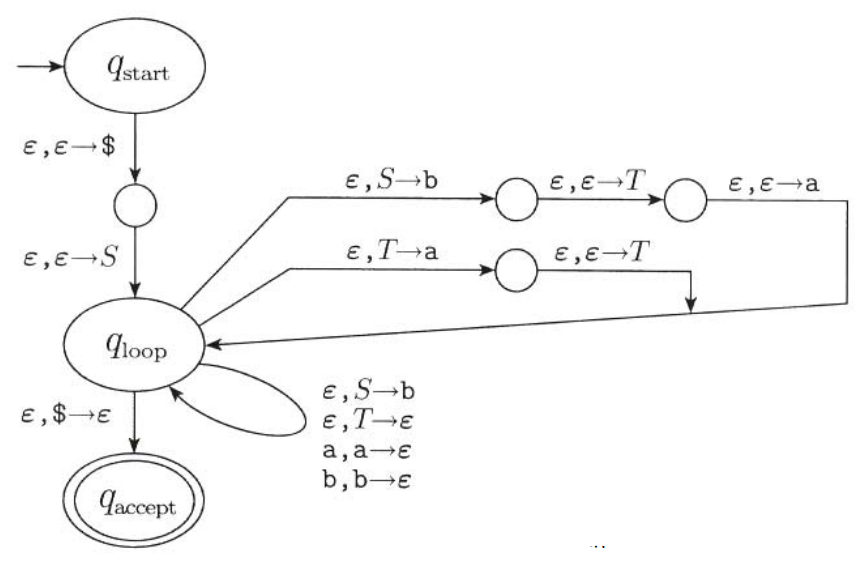
\includegraphics[width=0.6\textwidth]{images/es-CFG-implica-PDA.png}
    %\captionof{figure}{Diagramma di stato per un automa finito $M_2$}
\end{minipage}
\end{Example}

Ora dimostriamo la direzione inversa del Teorema \ref{thm:cfa-implica-pda}. Ora vogliamo trasformare un PDA in una CFG.

\begin{Lemma}{Automa a pila implica linguaggio context-free}{}
\textit{Se un linguaggio è riconosciuto da un automa a pila, allora esso è context-free.}

\begin{osservation}
Abbiamo un PDA $P$ e vogliamo costruire una CFG $G$ che genera tutte le stringhe che $P$ accetta. In altre parole, $G$ dovrebbe generare una stringa se quella stringa fa andare il PDA dal suo stato iniziale a uno stato accettante.

Per raggiungere questo risultato, progettiamo una grammatica che fa un pò in più. Per ciascuna coppia di stati $p$ e $q\in P$, la grammatica avrà una variabile $A_{pq}$. Questa variabile genera tutte le stringhe che possano portare $P$ da $p$ con pila vuota a $q$ con pila vuota. Si osservi che tali stringhe possono anche condurre $P$ da $p$ a $q$, indipendentemente dal contenuto della pila in $p$, lasciando la pila in $q$ nella stessa condizione in cui era in $p$.

Innanzitutto, semplifichiamo il nostro compito modificando leggermente $P$ per munirlo delle seguenti tre caratteristiche.
\begin{enumerate}
    \item Ha un unico stato accettante, $q_{accept}$.
    \item Svuota la sua pila prima di accettare.
    \item Ciascuna transizione inserisce un simbolo sulla pila (effettua un push) o ne elimina uno dalla pila (effettua un pop), ma non fa entrambe le azioni contemporaneamente.
\end{enumerate}

Dare a $P$ le caratteristiche 1 e 2 è facile. Per munirlo della caratteristica 3, sostituiamo ciascuna transizione che contemporaneamente elimina ed inserisce simboli con una sequenza di due transizioni che attraversa un nuovo stato, e sostituiamo ogni transizione che non elimina né inserisce simboli con una sequenza di due transizioni che inserisce e poi elimina un simbolo arbitrario della pila.

Per progettare $G$ in modo che $A_{pq}$ generi tutte le stringhe che portano $P$ da $p$ a $q$, iniziando e terminando con una pila vuota, dobbiamo capire come $P$ agisce su queste stringhe. Per ognuna di tali stringhe $x$, la prima mossa di $P$ su $x$ deve essere un push, poiché ogni mossa è un push o un pop e $P$ non può eliminare da una pila vuota. Analogamente, l'ultima mossa su $x$ deve essere un pop perché alla fine la pila deve essere vuota.

Durante la computazione di $P$ su $x$ si presentano due eventualità. O il simbolo eliminato alla fine è il simbolo che era stato inserito all'inizio, oppure no. Nel primo caso, la pila potrebbe essere vuota solo all'inizio e alla fine della computazione di $P$ su $x$. Altrimenti, il simbolo inizialmente inserito deve essere stato eliminato in qualche punto prima della fine di $x$ e quindi la pila si svuota in questo punto. Simuliamo la prima possibilità con la regola $A_{pq}\to aA_{rs}b$, dove $a$ è l'input letto nella prima mossa, $b$ è l'input letto nell'ultima mossa, $r$ è lo stato che segue $p$ ed $s$ è lo stato che precede $q$. Simuliamo la seconda possibilità con la regola $A_{pq}\to A_{pr}A_{rq}$, dove $r$ è lo stato in cui la pila diventa vuota.

\begin{demonstration}
Sia $P=(Q, \Sigma, \Gamma, \delta, q_{0} ,\{q_{accept}\})$ e costruiamo $G$. L'insieme delle variabili di $G$ è $\{A_{pq}|p,q \in Q\}$. La variabile iniziale è $A_{q_0,q_{accept}}$. Ora descriviamo le regole nei seguenti tre punti
\begin{enumerate}
    \item Per ogni $p, q, r,s \in Q$, $u \in\Gamma$ e $a, b\in \Sigma_{\epsilon}$, se $\delta(p, a, \epsilon)$ contiene $(r, u)$ e $\delta(s, b, u)$ contiene $(q, \epsilon)$, poni la $A_{pq}\to aA_{rs}b$ in $G$.
    \item Per ogni $p, q, r \in Q$ poni la regola $A_{pq}\to A_{pr}A_{rq}$ in $G$.
    \item Infine, per ogni $p \in Q$ poni la regola $A_{pp}\to \epsilon$ in $G$.
\end{enumerate}
Si può intuire questa costruzione dalle seguenti figure.
\end{demonstration}
\end{osservation}

\begin{minipage}{\textwidth}
    \centering
    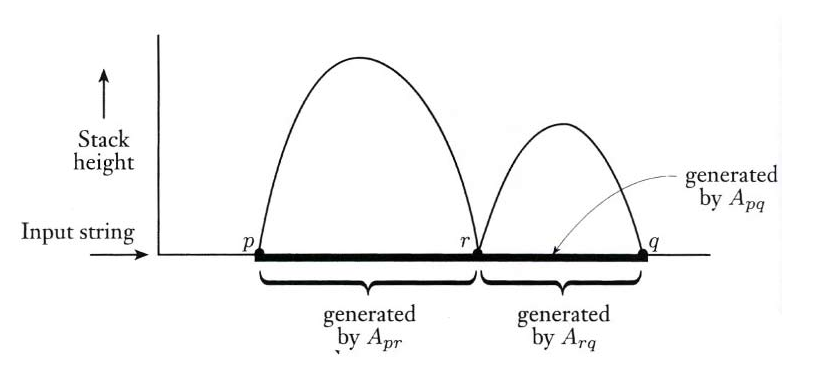
\includegraphics[width=0.49\textwidth]{images/pda-implica-cfg.PNG}
    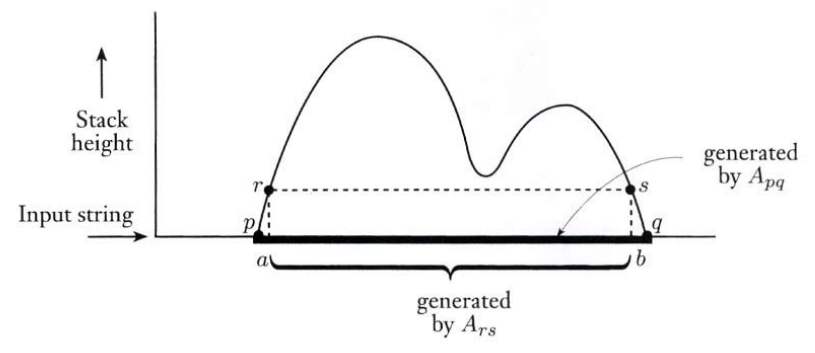
\includegraphics[width=0.49\textwidth]{images/pda-implica-cfg2.PNG}
    \captionof{figure}{PDA corrispondenti alle regole $A_{pq}\to A_{pr}A_{rq}$ e $A_{pq}\to aA_{rs}b$}
\end{minipage}

Ora proviamo che questa costruzione funziona dimostrando che $A_{pq}$ genera $x$ se e solo se $x$ porta $P$ da $p$ con la pila vuota a $q$ con la pila vuota. Consideriamo ogni direzione del "se e solo se" come un enunciato separato.
\end{Lemma}

\begin{Lemma}{$A_{pq}$ genera $x\implies$ $x$ porta $P$ da $p$ a $q$}{}
\textit{Se $A_{pq}$ genera $x$, allora $x$ può portare $P$ da $p$ con la pila vuota a $q$ con la pila vuota.}

Dimostriamo questo enunciato per induzione sul numero dei passi nella derivazione di $x$ da $A_{pq}$.
\begin{itemize}
    \item \textit{Passo base:} La derivazione è in un solo passo. Una derivazione in un solo passo deve usare una regola il cui lato destro non contenga variabili. Le uniche regole in $G$ con nessuna variabile sul lato destro sono $A_{pp}\to\epsilon$. Ovviamente, l'input $\epsilon$ porta $P$ da $p$ con la pila vuota a $p$ con la pila vuota quindi la base è dimostrata.
    \item \textit{Passo induttivo:} Assumiamo che l'enunciato sia vero per le derivazioni di lunghezza al più $k$, dove $k\geq 1$ e proviamo che esso è vero per le derivazioni di lunghezza $k + 1$.

    Supponiamo che $A_{pq}\Rightarrow^* x$ in $k + 1$ passi. Il primo passo in questa derivazione è $A_{pq}\Rightarrow aA_{rs}b$ oppure $A_{pq}\Rightarrow A_{pr} A_{rq}$. Trattiamo questi due casi separatamente.

    Nel primo caso, consideriamo la parte $y$ di $x$ che $A_{rs}$ genera, quindi $x = ayb$. Poiché $A_{rs}\Rightarrow^* y$ in $k$ passi, l'ipotesi induttiva ci dice che $P$ può andare da $r$ con la pila vuota a $s$ con la pila vuota. Poiché $A_{pq}\to aA_{rs} b$ è una regola di $G$, $\delta(p, a,\epsilon)$ contiene $(r, u)$ e $\delta(s, b, u)$ contiene $(q,\epsilon)$ per qualche simbolo di pila $u$. Quindi, se $P$ inizia in $p$ con la pila vuota, dopo aver letto $a$ può andare nello stato $r$ e inserire $u$ in cima alla pila. Poi, la lettura della stringa $y$ può portarlo in se lasciare $u$ sulla pila. In seguito dopo aver letto $b$ può andare nello stato $q$ ed eliminare $u$ dalla pila. Pertanto, $x$ può portare $P$ da $p$ con la pila vuota a $q$ con la pila vuota.

    Nel secondo caso, consideriamo le parti $y$ e z di $x$ che $A_{pr}$ e $A_{rq}$ rispettivamente generano, quindi $x = yz$. Poiché $A_{pr}\Rightarrow^* y$ in al più $k$ passi e $A_{rq}\Rightarrow^* z$ in al più $k$ passi, l'ipotesi induttiva ci dice che $y$ può portare $P$ può portare $P$ da $r$ a $q$, con la pila vuota all'inizio e alla fine della computazione. Quindi $z$ può portare $P$ da $p$ con la pila vuota a $q$ con la pila vuota. Questo completa la prova del passo induttivo.
\end{itemize}
\end{Lemma}

\begin{Lemma}{$x$ porta $P$ da $p$ a $q\implies$ $A_{pq}$ genera $x$}{}
Se $x$ può portare $P$ da $p$ con la pila vuota a $q$ con la pila vuota, $A_{pq}$ genera $x$.

Dimostriamo questo enunciato per induzione sul numero dei passi nella computazione di $P$ da $p$ a $q$ con pile vuote sull'input $x$.
\begin{itemize}
    \item \textit{Passo base:} La computazione è in 0 passi.

    Se una computazione è in 0 passi, essa inizia e termina nello stesso stato diciamo, $p$. Quindi dobbiamo mostrare che $A_{pp}\Rightarrow^* x$. $P$ non può leggere alcun carattere in 0 passi, quindi $x =\epsilon$. Per costruzione, $G$ ha la regola $A_{pp}\to\epsilon$, perciò la base è dimostrata.
    \item \textit{Passo induttivo:} Assumiamo l'enunciato vero per le computazioni di lunghezza al più $k$, dove $k\geq 0$ e dimostriamo che è vero per le computazioni di lunghezza $k + 1$.

    Supponiamo che $P$ abbia una computazione dove $x$ porta da $p$ a $q$ con pile vuote in $k + 1$ passi. O la pila è vuota solo all'inizio e alla fine di questa computazione oppure essa si svuota anche altrove.

    Nel primo caso, il simbolo che è stato inserito nella prima mossa deve essere lo stesso simbolo che è stato rimosso nell'ultima mossa. Chiamiamo $u$ questo simbolo. Sia $a$ il simbolo di input letto nella prima mossa, $b$ il simbolo di input letto nell'ultima mossa, $r$ lo stato dopo la prima mossa ed $s$ lo stato prima dell'ultima mossa. Allora $\delta(p, a, \epsilon)$ contiene $(r, u)$ e $\delta(s, b, u)$ contiene $(q, \epsilon)$ e quindi la regola $A_{pq}\to aA_{rs}b$ è in $G$. Sia $y$ la parte di $x$ senza $a$ e $b$, quindi $x = ayb$. L'input $y$ può portare $P$ da $r$ a $s$ senza toccare il simbolo $u$ che è sulla cima della pila e quindi $P$ può andare dar con una pila vuota a $s$ con una pila vuota sull'input $y$. Abbiamo eliminato il primo e l'ultimo passo dei $k + 1$ passi nella computazione iniziale su $x$, perciò la computazione su $y$ ha $(k + 1) - 2 = k - 1$ passi. Quindi l'ipotesi induttiva ci dice che $A_{rs}\Rightarrow^* y$. Allora $A_{pq}\Rightarrow^* x$.

    Nel secondo caso, sia $r$ uno stato in cui la pila oltre che all'inizio o alla fine della computazione su $x$. Allora le parti della computazione da $p$ a $r$ e da $r$ a $q$ contengono al più $k$ passi. Sia $y$ l'input letto nella prima parte e sia $z$ l'input letto nella seconda parte. L'ipotesi induttiva ci dice che $A_{pr}\Rightarrow^* y$ e $A_{rq}\Rightarrow^* z$. Poiché la regola $A_{pq}\to A_{pr}A_{rq}$ è in $G$, $A_{pq}\Rightarrow^* x$ e la dimostrazione è completa.
\end{itemize}
\end{Lemma}

\section{Linguaggi non context-free}
In questa sezione presentiamo una tecnica per dimostrare che alcuni linguaggi non sono context-free. A questo punto presentiamo un pumping lemma per i linguaggi context-free. Esso stabilisce che per ogni linguaggio context-free esiste un particolare valore chiamato la lunghezza del pumping tale che tutte le stringhe più lunghe nel linguaggio possono essere "iterate". Significa che la stringa può essere divisa in cinque parti in modo tale che la seconda e la quarta parte possono insieme essere replicate un numero qualsiasi di volte ottenendo una stringa che appartiene ancora al linguaggio.

\subsection{Pumping lemma per i linguaggi context-free}
\begin{Thm}{Pumping lemma per i linguaggi context-free}{}
\textit{Se $A$ è un linguaggio context-free, allora esiste un numero $p$ (la lunghezza del pumping) tale che, se $s$ è una qualsiasi stringa in $A$ di lunghezza almeno $p$, allora $s$ può essere divisa in cinque parti $s = uvxyz$ che soddisfano le condizioni}
\begin{enumerate}
    \item per ogni $i\geq 0$, $uv^ixy^iz\in A$,
    \item $|vy|>0$ e
    \item $|vxy|\leq p$.
\end{enumerate}

Quando s è divisa in $uvxyz$, la condizione 2 afferma che $u$ oppure $y$ non è la stringa vuota. Altrimenti il teorema sarebbe banalmente vero. La condizione 3 afferma che le parti $v$, $x$ e $y$ insieme hanno lunghezza al più $p$.

\begin{osservation}
Sia $A$ un CFL e sia $G$ una CFG che lo genera. Dobbiamo mostrare che ogni stringa sufficientemente lunga $s$ in $A$ può essere iterata e restare in $A$. L'idea dietro questa strategia è semplice.

Sia $s$ una stringa molto lunga in $A$. Poiché $s$ è in $A$, essa è derivabile da $G$ e quindi ha un albero sintattico. L'albero sintattico per $s$ deve essere molto alto perché $s$ è molto lunga. Cioè l'albero sintattico deve contenere un cammino lungo dalla variabile alla radice dell'albero a uno dei simboli terminali su una foglia. Per il principio della piccionaia, qualche simbolo di variabile $R$ si deve ripetere in questo cammino lungo. Questa ripetizione ci permette di sostituire il sottoalbero sotto la seconda occorrenza di $R$ con il sottoalbero sotto la prima occorrenza di $R$ e ottenere ancora un albero sintattico consentito. Pertanto, possiamo dividere $s$ in cinque parti $uvxyz$ e possiamo replicare il secondo e quarto pezzo e ottenere una stringa ancora nel linguaggio. In altre parole, $uv^ixy^iz$ è in $A$ per ogni $i\geq 0$.
\end{osservation}

\begin{minipage}{\textwidth}
    \centering
    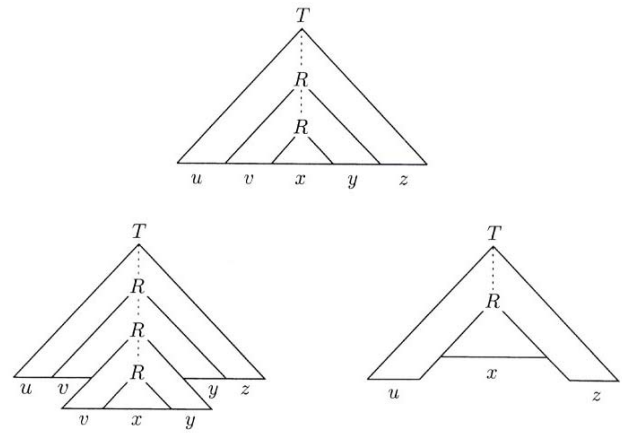
\includegraphics[width=0.6\textwidth]{images/alberi-sintattici.PNG}
    %\captionof{figure}{}
\end{minipage}

Veniamo ora ai dettagli per ottenere tutte e tre le condizioni del pumping lemma. Mostreremo anche come calcolare la lunghezza del pumping $p$.

\begin{demonstration}
Sia $G$ una CFG per il CFL $A$. Sia $b$ il massimo numero di simboli nel lato destro di una regola (assumiamo che sia almeno 2). Sappiamo che, in ogni albero sintattico costruito usando questa grammatica, un nodo non può avere più di $b$ figli. In altre parole, ci sono al più $b$ foglie in un passo dalla variabile iniziale; ci sono al più $b ^ 2$ foglie in 2 passi dalla variabile iniziale; e ci sono al più $b ^ h$ foglie in $h$ passi dalla variabile iniziale. Quindi, se l'altezza dell'albero sintattico è al più $h$, la lunghezza della stringa generata è al più $b ^ h$. Viceversa, se una stringa generata ha lunghezza maggiore o uguale a $b ^ h + 1$ ciascuno dei suoi alberi sintattici deve avere un'altezza maggiore o uguale a $h + 1$. Sia $|V|$ il numero delle variabili in $G$. Poniamo $p$, la lunghezza del pumping, uguale a $b^{(|V| + 1)}$. Ora se $s$ è una stringa in $A$ e la sua lunghezza è maggiore o uguale a $p$, il suo albero sintattico deve avere altezza maggiore o uguale a $|V| + 1$ poiché $b^{(|V| + 1)}\geq b^{|V|} + 1$.

Per vedere come iterare una tale stringa $s$, sia $\tau$ uno dei suoi alberi sintattici. Se $s$ ha diversi alberi sintattici, scegliamo un albero sintattico $\tau$ che abbia il più piccolo numero di nodi. Sappiamo che $\tau$ deve avere altezza maggiore o uguale a $|V| + 1$ quindi il suo cammino più lungo dalla radice a una foglia ha lunghezza almeno $|V| + 1$. Questo cammino ha almeno $|V| + 2$ nodi; uno etichettato da un terminale, gli altri etichettati da variabili. Quindi questo cammino ha almeno $|V| + 1$ variabili. Poiché $G$ ha solo $|V|$ variabili, qualche variabile $R$ è presente più di una volta su questo cammino. Per un utilizzo successivo, scegliamo $R$ in modo che sia una variabile che si ripete tra le $|V| + 1$ variabili più in basso su questo cammino.

Dividiamo $s$ in $uvxyz$ come nella figura. Ogni occorrenza di $R$ ha un sottoalbero sotto essa che genera una parte della stringa $s$. L'occorrenza più in alto di $R$ ha un sottoalbero più grande e genera $vxy$, mentre l'occorrenza più in basso genera solo $x$ con un sottoalbero più piccolo. Entrambi questi sottoalberi sono generati dalla stessa variabile, quindi possiamo sostituire l'uno con l'altro e ottenere ancora un albero sintattico corretto. Sostituire ripetutamente il più piccolo con il più grande fornisce gli alberi sintattici per le stringhe $uv^ixy^iz$ per ogni $i > 1$. Sostituire il più grande con il più piccolo genera la stringa $uxz$. Questo dimostra la condizione 1 del lemma. Ora veniamo alle condizioni 2 e 3.

Per ottenere la condizione 2, dobbiamo essere sicuri che $v$ e $y$ non sono entrambe $\epsilon$. Se lo fossero, l'albero sintattico ottenuto sostituendo il più piccolo sottoalbero al più grande avrebbe meno nodi di $\tau$ e genererebbe ancora $s$. Questo non è possibile perché abbiamo scelto $\tau$ in modo che sia un albero sintattico per $s$ con il più piccolo numero di nodi. Questa è la ragione per aver selezionato così $\tau$.

Per ottenere la condizione 3, dobbiamo essere sicuri che $vxy$ ha lunghezza al più $p$. Nell'albero sintattico per $s$ l'occorrenza più in alto di $R$ genera $vxy$. Abbiamo scelto $R$ in modo che entrambe le occorrenze di essa cadano nelle $|V| + 1$ variabili più in basso del cammino e abbiamo scelto il più lungo cammino nell'albero sintattico, in modo che il sottoalbero in cui $R$ genera $vxy$ sia alto al più $|V| + 1$. Un albero con questa altezza può generare una stringa di lunghezza al più $b ^{(|V| + 1)} = p$.
\end{demonstration}
\end{Thm}

\begin{Example}{Pumping lemma per i linguaggi context-free}{}
\textit{Consideriamo il linguaggio $L = \{0^n1^n2^n| n\geq0\}$ e dimostriamo che non è un CFL.}

Supponiamo per assurdo che $L$ sia un CFL. In tal caso, ne segue che per esso debbia
valere il pumping lemma, dove $p$ è la lunghezza del pumping.
Consideriamo quindi la stringa $w := 0^p1^p2^p$. Poiché $|w|\geq p$, possiamo suddividerla in cinque sottostringhe $u, v, x, y, z\in \Sigma^*$ tali che $w = uvxyz$. 

Poiché la terza condizione del pumping lemma impone che $|vxy| \leq p$, le uniche
possibilità sono:
\begin{enumerate}
    \item Se $vxy = 0^m$ con $1 \leq m \leq p$, si ha che $u = 0^h$ e $z = 0^{p-m-h}1^p2^p$, dove $1 \leq m + h \leq p$. Inoltre, poiché la seconda condizione impone che $|vy| > 0$, si ha che $v$ e/o $y$ contengono almeno uno 0.
    \item Se $vxy = 1^m$ con $1 \leq m \leq p$, si ha che $u = 0^p1^h$ e $z = 1^{p-m-h}2^p$, dove $1 \leq m + h \leq p$. Inoltre, poiché la seconda condizione impone che $|vy| > 0$, si ha che $v$ e/o $y$ contengono almeno un 1.
    \item Se $vxy = 2^m$ con $1 \leq m \leq p$, si ha che $u = 0^p1^p$ e $z = 2^{p-m-h}$, dove $2\leq m + h \leq p$. Inoltre, poiché la seconda condizione impone che $|vy| > 0$, si ha che $v$ e/o $y$ contengono almeno un 2.
    \item Se $vxy = 0^m1^h$ con $1 \leq m + h \leq p$, si ha che $u = 0^{p-m}$ e $z = 1^{p-h}2^p$. Inoltre, poiché la seconda condizione impone che $|vy| > 0$, si ha che $v$ contiene almeno uno 0 e/o $y$ contiene almeno un 1.
    \item Se $vxy = 1^m2^h$ con $1 \leq m + h \leq p$, si ha che $u = 0^p1^{p-m}$ e $z = 2^{p-h}$. Inoltre, poiché la seconda condizione impone che $|vy| > 0$, si ha che $v$ contiene almeno uno 1 e/o $y$ contiene almeno un 2.
\end{enumerate}

In tutti i casi possibili descritti, risulta automatico che 
\begin{equation*}
    \nexists n\geq0|n=|uv^0xy^0z|_0=|uv^0xy^0z|_1=|uv^0xy^0z|_2\implies uv^0xy^0z\notin L
\end{equation*}
contraddicendo quindi la prima condizione del pumping lemma. Di conseguenza, ne segue necessariamente che L non è un CFL.
\end{Example}

\begin{Example}{Pumping lemma per i linguaggi context-free}{}
\textit{Consideriamo il linguaggio $L = \{ww | w \in \{0, 1\}^*\}$ e dimostriamo che non è un CFL.}

Supponiamo per assurdo che $L$ sia un CFL. In tal caso, ne segue che per esso debbia valere il pumping lemma, dove $p$ è la lunghezza del pumping. Consideriamo quindi la stringa $w := 0^p1^^p0^p1^p$. Poiché $|w| \geq p$, possiamo suddividerla in cinque sottostringhe $u, v, x, y, z \in\Sigma^*$ tali che $w = uvxyz$. 

Poiché la terza condizione del pumping lemma impone che $|vxy| \leq p$, le uniche possibilità sono:
\begin{enumerate}
    \item Se $u = 0^h$, $vxy = 0^m$ e $z = 0^{p-m-h}1^p0^p1^p$, dove $1 \leq m + h \leq p$, poiché la seconda condizione impone che $|vy| > 0$, si ha che $v$ e/o $y$ contengono almeno uno 0, dunque si ha che: 
    \begin{equation*}
    \exists k < m | v^0xy^0 = 0^k \implies uv^0xy^0z = 0^h0^k0^{p-m-h}1^p0^p1^p = 0^{p-m+k}1^p0^p1^p        
    \end{equation*}
    dove $k < m \implies p - m - k < p$ e dunque che $uv^0xy^0z \notin L$.
    \item Se $u = 0^p1^p0^h$, $vxy = 0^m$ e $z = 0^{p-m-h}1^p$, dove $1 \leq m+h \leq p$, procedendo analogamente al caso (1) otteniamo che $uv^0xy^0z \notin L$.
    \item Se $u = 0^p1^h$, $vxy = 1^m$ e $z = 1^{p-m-h}0^p1^p$, dove $1 \leq m+h \leq p$, procedendo analogamente al caso (1) otteniamo che $uv^0xy^0z \notin L$.
    \item Se $u = 0^p1^p0^p1^h$, $vxy = 1^m$ e $z = 1^{p-m-h}$, dove $1 \leq m+h \leq p$, procedendo analogamente al caso (1) otteniamo che $uv^0xy^0z \notin L$.
    \item Se $u = 0^{p-h}$, $vxy = 0^h1^m$ e $z = 1^{p-m}0^p1^p$, dove $1 \leq m + h \leq p$, poiché la seconda condizione impone che $|vy| > 0$, si ha che $v$ contiene almeno uno 0 e/o $y$ contiene almeno un 1, dunque si ha che:
    \begin{equation*}
        \exists j < h, j < m | v^0xy^0 = 0^j1^k \implies uv^0xy^0z = 0^{p-h}0^j1^k1^{p-m}0^p1^p = 0^{p-h+j}1^{p-m+k}0^p1^p
    \end{equation*}
    dove $j < h, k < m \implies p-h+j, p-m+k < p$ e dunque che $uv^0xy^0z \notin L$.
    \item Se $u = 0^p1^p0^{p-h}$, $vxy = 0^h1^m$ e $z = 1^{p-m}$, dove $1 \leq m+h \leq p$, procedendo analogamente al caso (5) otteniamo che $uv^0xy^0z \notin L$.
    \item Se $u = 0^p1^{p-h}$, $vxy = 1^h0^m$ e $z = 0^{p-m}1^p$, dove $1 \leq m + h \leq p$, poiché la seconda condizione impone che $|vy| > 0$, si ha che $v$ contiene almeno uno 1 e/o $y$ contiene almeno un 0, dunque si ha che:
    \begin{equation*}
        \exists j < h, j < m | v^0xy^0 = 1^j0^k \implies uv^0xy^0z = 0^p1^{p-h}1^j0^k0^{p-m}1^p = 0^p1^{p-h+j}0^{p-m+k}1^p
    \end{equation*}
    dove $j < h, k < m \implies p-h+j, p-m+k < p$ e dunque che $uv^0xy^0z \notin L$.
\end{enumerate}

Di conseguenza, poiché il pump down non può essere effettuato nè in un blocco di soli 0 o soli 1 (casi 1, 2, 3, 4), nè a cavallo tra degli 0 ed 1 (casi 5, 6), nè al centro della stringa (caso 7), ne segue che la prima condizione del pumping lemma venga contraddetta. Di conseguenza, ne segue necessariamente che $L$ non è un CFL.
\end{Example}

\begin{Example}{Chiusura della concatenazione in CFL}{}
\textit{Consideriamo i seguenti linguaggi $L_1 = \{0^n1^n| n\geq N\}$ e $L_2 = \{1^m2^m | m\geq0\}$.}

Consideriamo quindi le due grammatiche:
\begin{gather*}
G_1 : A \to 0A1 | \epsilon\\
G_2 : B \to 1A0 | \epsilon  
\end{gather*}
tali che $L_1 = L(G_1)$ e $L_2 = L(G_2)$.

La grammatica $G$ tale che $L(G) = L_1\cup L_2$, corrisponderà a:
\begin{gather*}
G : S \to A | B\\
A \to 0A1 | \epsilon\\
B \to 0B1 | \epsilon 
\end{gather*}
La grammatica $G'$ tale che $L(G') = L_1\circ L_2$, corrisponderà a:
\begin{gather*}
G : S \to AB\\
A \to 0A1 | \epsilon\\
B \to 0B1 | \epsilon
\end{gather*}
\end{Example}

\begin{Example}{Non chiusura del complemento in CFL}{}
\textit{Consideriamo il seguente linguaggio $L = \{a, b\}^* - \{ww | w \in \{a, b\}^*\}$}.

Consideriamo quindi la seguente grammatica 
\begin{gather*}
G : S \to A | B | AB | BA\\
A \to a | aAa | aAb | bAa | bAb\\
B \to b | aBa | aBb | bBa | bBb
\end{gather*}

Data $x \in L$ tale che $|x|$ sia dispari, notiamo che se il simbolo centrale di $x$ è $a$, allora $S \implies A \implies^* x$, se il simbolo centrale di $x$ è $b$, allora $S \implies B
\implies^* x$, dunque ne segue che $x \in L(G)$.
Viceversa, data $x \in L(G)$ tale che $|x|$ sia dispari, ne segue immediatamente che $\nexists w \in \{a, b\}^* | x = ww \implies x \in L$. Sia quindi $x \in L$ tale che $|x|$ sia pari.
Dati $x_1,..., x_n \in {a, b}$ tali che $x = x_1...xn$, ne segue che:
\begin{equation*}
    x \in L \implies \exists i \in [1, n] | xi\neq x_{\frac{n}{2}+i}
\end{equation*}
Siano quindi $u := x_1 . . . x_{2i-1}$ e $v := x_{2i}...x_n$. Notiamo che il simbolo centrale di
$u$ corrisponde a $x_{\frac{1+2i-1}{2}}$, mentre quello di $v$ corrisponde a $x_{\frac{2i+n}{2}}=x_{\frac{n}{2}+i}$, da cui traiamo che:
\begin{equation*}
    x_i\neq x_{\frac{n}{2}+i}\implies x_{\frac{1+2i-1}{2}}=x_i\neq x_{\frac{2i+n}{2}}\implies u\neq v    
\end{equation*}
Inoltre, notiamo che $|u|$ e $|v|$ siano dispari, dunque si ha che $u, v \in L(G)$. Di
conseguenza, otteniamo che:
\begin{equation*}
    S \implies AB\implies^* uv = x \textit{ oppure } S \implies BA \implies^* uv = x    
\end{equation*}
implicando quindi che $x \in L(G)$.

Sia quindi $x \in L(G)$ tale che $|x|$ sia pari.
Poiché $|x|$ è pari, ne segue necessariamente che:
\begin{equation*}
S \implies AB \implies^* x \textit{ oppure } S \implies BA \implies^* x    
\end{equation*}
Poiché i due casi sono analoghi, senza perdita di generalità consideriamo il caso in
cui $S \implies AB \implies^* x$.
Siano quindi $u := x_1 . . . x_k$ e $v := x_{k+1} . . . v_n$ tali che $x = uv$, $S \implies A
\implies^* u$ e $S \implies B\implies^* v$.
Poiché $S \implies A \implies^* u$ e $S \implies B \implies^* v$, otteniamo che: $|u| = k$ e $|v| = n - k$ sono dispari; $S \implies A \implies^* u$ implica che il simbolo centrale di $u$ sia $a$, ossia che $x_{\frac{1+k}{2}}= a$; $S \implies B\implies^* v$ implica che il simbolo centrale di $v$ sia $b$, ossia che $x_{\frac{k+1+n}{2}}= b$.
Siano quindi che $w := w_1 . . . w_h$ e $w':= w'_1. . . w'_h$ tali che $|w| = |w'| = h$ e che $u = ww'$, implicando dunque che $h = \frac{n}{2}$. Per il risultato precedente, ne segue automaticamente che:
\begin{equation*}
    w_{\frac{1+h}{2}}=x_{\frac{1+k}{2}}= a\neq b=x_{\frac{k+1+n}{2}}=w'_{\frac{1+h}{2}}\implies w\neq w' \implies x = ww' \in L
\end{equation*}
Dunque, abbiamo ottenuto $L = L(G) \in CFL$. Il complemento di tale linguaggio risulta essere $L = \{ww | w \in \{a, b\}^*\}$, il quale abbiamo già dimostrato non essere un linguaggio acontestuale. Di conseguenza, concludiamo che $L \in CFL$, ma $\overline{L} \notin CFL$.
\end{Example}